\documentclass[12pt,titlepage]{beamer}
\usepackage{pdfpcnotes}
% language stuff
\usepackage{german}           % deutsche Überschriften etc.
\usepackage[utf8]{inputenc} % direkte Einbgabe von Umlauten

% Layout-Einstellungen
\usepackage{parskip}          % Abstand statt Einrückung
\frenchspacing                % no extra space after periods
\usepackage{parskip}          % paragraph gaps instead of indentation
\usepackage{times}            % default font Times
\tolerance=9000               % avoid words across right border
% miscellaneous<
\usepackage{hhline}           % double lines in tables
\usepackage{amsfonts}         % real numbers etc.
\usepackage[rightcaption]{sidecap} % figure captions on the right (optional)
\usepackage{hyperref}         % for URLs
\usepackage{listings}         % for code samples
 \lstset{breaklines=true,tabsize=1}
\usepackage{etoolbox}
\usepackage{multirow}
\usepackage{tabularx}
\usepackage{amsmath}
\usepackage{multirow}
\usepackage{pbox}
\usepackage{graphicx}
\usepackage[vlined]{algorithm2e}
\usepackage{svg}
\usepackage{tikz}

\lstset{
basicstyle=\footnotesize,
frame=single
}


\definecolor{HIGHLIGHTCOLOR}{rgb}{0.13333333333333333,0.8156862745098039,0.09019607843137255}



\defbeamertemplate{section page}{mine}[1][]{%
  \begin{centering}
    {\usebeamerfont{section name}\usebeamercolor[fg]{section name}#1}
    \vskip1em\par
    \begin{beamercolorbox}[sep=12pt,center]{part title}
      \usebeamerfont{section title}\insertsection\par
    \end{beamercolorbox}
  \end{centering}
}

\AtBeginSection{\setbeamertemplate{section page}[mine]\frame{\sectionpage}}


\makeatletter
\patchcmd{\insertverticalnavigation}%
{\ifx\beamer@nav@css\beamer@hidetext{\usebeamertemplate{section in sidebar}}\else{\usebeamertemplate{section in sidebar shaded}}\fi}%
{{\usebeamertemplate{section in sidebar}}}{}{}
\makeatother



% Hier bei Bedarf die Seitenränder einstellen
%\geometry{a4paper}
\usetheme{Hannover}
\usecolortheme{rose}
\begin{document}
	\title{Netzoptimierung und Lernalgorithmen für Neuronale Netze}
	\author{Michael Kämmerer}
	\date{\today}
	\institute{}
%------------------------------------------------Folie1----------------------------------------------------------
	\begin{frame}
		\maketitle
	\end{frame}
	\section{Grundlagen}
	\subsection{Allgemeiner Aufbau neuronaler Netze}
		
	\begin{frame}
	\frametitle{Allgemeiner Aufbau neuronaler Netze}
	Künstliche neuronale Netze versuchen Lernmodelle des Gehirns nachzubilden.
	
	Es existieren verschiedenste Lernverfahren zum trainieren von neuronalen Netzen.
	
	Neuronale Netze können vielseitig eingesetzt werden, zum Beispiel in der Mustererkennung.
	
	\end{frame}
	\begin{frame}
	\frametitle{Allgemeiner Aufbau neuronaler Netze}
Zur Abbildung der funktionsweise existiert ein mathematisches Modell:
\begin{figure}[H]
	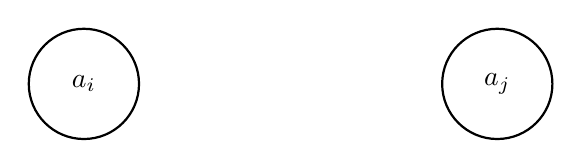
\begin{tikzpicture}[scale=0.7]
	
	\draw[thick](3.5,0)circle(1) node{$a_i$};
	
	\draw[thick](11,0)circle(1) node{$a_j$};
	
	\end{tikzpicture}
\end{figure}
1. Jedes Neuron hat einen Aktivierungszustand $a_i(t)$ zum Zeitpunkt t.
\end{frame}
\begin{frame}
\frametitle{Allgemeiner Aufbau neuronaler Netze}
\begin{figure}[H]
	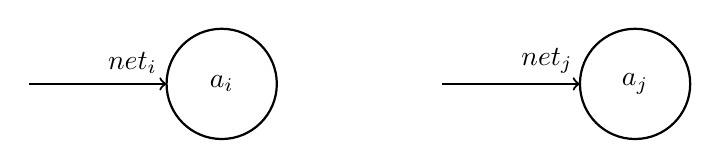
\begin{tikzpicture}[scale=0.7]
	\draw[->,thick](0,0)--(2.5,0)node[above right, midway]{$net_i$};
	\draw[thick](3.5,0)circle(1) node{$a_i$};
	\draw[->,thick](7.5,0)--(10,0)node[above right, midway]{$net_j$};
	\draw[thick](11,0)circle(1) node{$a_j$};
	\end{tikzpicture}
\end{figure}
2. Jedes Neuron hat eine Aktivierungsfunktion $f_{act}$ zur Berechnung eines neuen Aktivierungszustandes aus er Eingabe $net_i$ und eines Schwellwerts.
\end{frame}
\begin{frame}
\frametitle{Allgemeiner Aufbau neuronaler Netze}
\begin{figure}[H]
	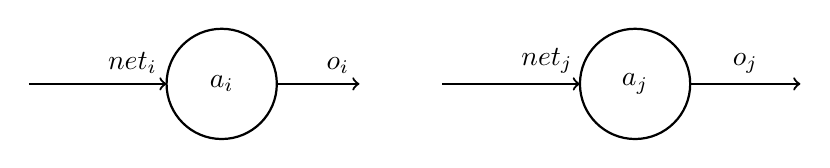
\begin{tikzpicture}	[scale=0.7]
	\draw[->,thick](0,0)--(2.5,0)node[above right, midway]{$net_i$};
	\draw[thick](3.5,0)circle(1) node{$a_i$};
	\draw[->,thick](4.5,0)--(6,0)node[above left]{$o_i$};
	\draw[->,thick](7.5,0)--(10,0)node[above right, midway]{$net_j$};
	\draw[thick](11,0)circle(1) node{$a_j$};
	\draw[thick,->](12,0)--(14,0) node[above,midway]{$o_j$};
	\end{tikzpicture}
\end{figure}
3. Jedes Neuron hat eine Ausgabefunktion $f_{out}$ die aus dem Aktivierungszustand die Ausgabe $o$ des Neurons berechnet.
\end{frame}
\begin{frame}
\frametitle{Allgemeiner Aufbau neuronaler Netze}
\begin{figure}[H]
	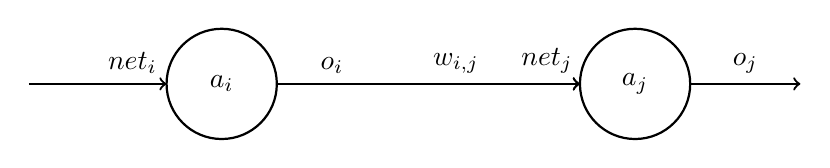
\begin{tikzpicture}[scale=0.7]
	\draw[->,thick](0,0)--(2.5,0)node[above right, midway]{$net_i$};
	\draw[thick](3.5,0)circle(1) node{$a_i$};
	\draw[thick](4.5,0)--(5.5,0)node[above]{$o_i$};
	\draw[->,thick](5.5,0)--(10,0)node[midway, above]{$w_{i,j}$};
	\draw[->,thick](7.5,0)--(10,0)node[above right, midway]{$net_j$};
	\draw[thick](11,0)circle(1) node{$a_j$};
	\draw[thick,->](12,0)--(14,0) node[above,midway]{$o_j$};
	\end{tikzpicture}
\end{figure}
4. Die Neuronen sind über ein Netzwerk aus Synapsen $w_{ij}$ miteinander verbunden.
\end{frame}
\begin{frame}
\frametitle{Allgemeiner Aufbau neuronaler Netze}
	\begin{figure}[H]
	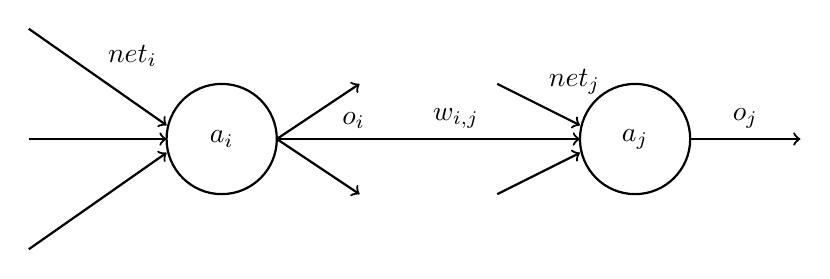
\begin{tikzpicture}	[scale=0.7]
	\draw[->,thick](0,0)--(2.5,0);
	\draw[->,thick](0,2)--(2.5,0.25)node[above right, midway]{$net_i$};
	\draw[->, thick](0,-2)--(2.5,-0.25);
	\draw[thick](3.5,0)circle(1) node{$a_i$};
	\draw[thick](4.5,0)--(5.5,0)node[above right]{$o_i$};
	\draw[->,thick](4.5,0)--(6,1);
	\draw[->,thick](4.5,0)--(6,-1);
	\draw[->,thick](5.5,0)--(10,0)node[midway, above]{$w_{i,j}$};
	\draw[->,thick](8.5,1)--(10,0.25)node[above right, midway]{$net_j$};
	\draw[->,thick](8.5,-1)--(10,-0.25);
	\draw[thick](11,0)circle(1) node{$a_j$};
	\draw[thick,->](12,0)--(14,0) node[above,midway]{$o_j$};
	\end{tikzpicture}
\end{figure}
5. Eine Propagierungsfunktion, die aus den Ausgaben anderer Neuronen die Eingabe eines Neurons berechnet.

6. Eine Lernregel.
\end{frame}
	\subsection{Backpropagation}
	\begin{frame}
	\frametitle{Backpropagation}
	Backpropagation ist ein überwachtes Lernverfahren, d.h. eine Ist-Ausgabe wird mit einer Soll-Ausgabe verglichen.
	
	Einfaches Prinzip: Propagiere ein Muster durchs Netz, Vergleiche Ausgaben, propagiere den Fehler rückwärts durchs Netz und passe Gewichte an um diesen zu minimieren
	\end{frame}
	\subsection{Markov-Ketten}
	\begin{frame}
	\frametitle{Markov-Ketten}
	Stochastischer Prozess zur Beschreibung der zeitlichen Abfolge von zufälligen Vorgängen Vorgängen. 	
	
	Wichtigste Eigenschaft: Der Zustand zu einem Zeitpunkt ist nur vom Zustand davor abhängig
		\end{frame}
	\subsection{Hopfield Netze}
	\begin{frame}
	\frametitle{Hopfield Netze}
	\begin{figure}[H]
	\center
	\includesvg[width=3cm]{Hopfield}
	\label{HopfieldNetz}
	\end{figure}
	Alle Neuronen sind miteinander verbunden und feuern wenn ein Schwellwert $\theta$ überschritten wird. Ziel ist es eine Energiefunktion zu minimieren:
	$$
	E = -\frac{1}{2}\sum_{i\neq j}{w_{ij}{s_i}{s_j}}+\sum_i{\theta_i\ s_i}
	$$
	\end{frame}
	\subsection{Boltzmann Maschinen}
	
	\begin{frame}
	\frametitle{Boltzmann Maschinen}
	\begin{figure}[H]
	\center
	\includesvg[width=3cm]{BM}
	\label{Boltzmannmaschine}
	\end{figure}
	Neuronen Aktivieren sich über Wahrscheinlichkeiten statt Schwellwerten. Es gibt sichtbare und versteckte Neuronen.
	Auch hier wird eine Energiefunktion minimiert:
	$$
	E = -\left(\sum_{i<j} w_{ij} \, s_i \, s_j + \sum_i \theta_i \, s_i \right)$$
	\pnote{sichtbar: Hat Eingabe von außen}
	\pnote{unsichtbar: Hat KEINE Eingabe von außen}
	\end{frame}
	\begin{frame}
	\frametitle{Boltzmann Maschinen}
	Training findet in zwei Phasen statt:
	\begin{itemize}
	\item positive Phase: Sichtbare Neuronen bekommen Trainingsdaten als Eingabe
	\item negative Phase: sichtbare Neuronen sind zufällig initialisiert
	\end{itemize}
	Beide Phase laufen bis sich ein Gleichgewichtszustand einstellt und es ergibt sich als Differenz:
	$$
G = \sum_{v}{P^{+}(v)\ln\left({\frac{P^{+}(v)}{P^{-}(v)}}\right)}
$$
Daraus folgt diese Lernregel:
$$
\frac{\partial{G}}{\partial{w_{ij}}} = -\frac{1}{R}[p_{ij}^{+}-p_{ij}^{-}]
$$
	\end{frame}
	\subsection{Eingeschränkte Boltzmann Maschinen}
	\begin{frame}
	\frametitle{Eingeschränkte Boltzmann Maschinen}
	\begin{figure}[H]
	\center
	\includesvg[width=3cm]{RBM}
	\end{figure}
	Versteckte und sichtbare Neuronen werden in Ebenen unterteilt ohne Verbindungen innerhalb einer Ebene. Auch hier gibt es eine Energiefunktion:
	$$
E(\vec{v},\vec{h})= - \sum_{i \in visible} a_iv_i- \sum_{j \in hidden} b_j h_j - \sum_{i,j} v_i h_j w_{ij}
$$
	\end{frame}
	\begin{frame}
	\frametitle{Eingeschränkte Boltzmann Maschinen}
	Die Wahrscheinlichkeit dass ein versteckter Knoten auf 1 gesetzt wird:
	$$p(h_j = 1 | \vec{v}) = \sigma (b_j + \sum_{i} v_i w_{ij})$$
	$\sigma(x)$ ist die sigmoide Funktion $1/(1+e^{-x})$
	Analog gilt das gleiche für sichtbare Knoten
	\end{frame}
	
	\begin{frame}
	\frametitle{Eingeschränkte Boltzmann Maschinen}
	Als Lernregel ergibt sich:
	$$\Delta w_{ij} = \epsilon\left( \langle v_i h_j \rangle_{data} - \langle v_i h_j \rangle_{model} \right)$$
	Zum besseren Verständnis schaut man sich die Änderungen nach einem Schritt an:
	$$
	\frac{\Delta \log p(v^0)}{\Delta w^{00}_{ij}} = <h^0_j(v^0_i-v_i^1)>
	$$
	Und danach für viele Schritte:
	\begin{flalign*}
\frac{\Delta \log p(v)}{\Delta w_{ij}}&=<h^0_j(v^0_i-v_i^1)>\\\nonumber
&+<v^1_i(h^0_j-h_j^1)>\nonumber\\
&+<h^1_j(v^1_i-v_i^2)> + \dots\nonumber
\end{flalign*}
\end{frame}

\begin{frame}
\frametitle{Eingeschränkte Boltzmann Maschinen}
Zum berechnen von $\langle v_i h_j \rangle_{model}$ verwendet man Gibbs-Sampling
\begin{figure}[H]
	\center
	\includesvg[width=\textwidth]{Markov}
	
	\end{figure}
	\end{frame}
	\subsection{Kontrastive Divergenz}
	\begin{frame}
	\frametitle{Kontrastive Divergenz}
	Gibbs Sampling dauert sehr lange und die Markov-Kette wird immer unabhängiger vom Modell der Eingabedaten je länger sie läuft.
	
	Lösung: Mache immer nur einen Gibbs Sampling Schritt und berechne dann die Gewichte neu
	
	Neue Lernregel:
	
	$$\Delta w_{ij} = \epsilon \left( \langle v_i h_j\rangle_{data} - \langle v_i h_j \rangle_{recon}\right)$$
	
	
	\end{frame}
	\begin{frame}
	\frametitle{Kontrastive Divergenz}
	Problem der neuen Lernregel:
	Man kann zwar zeigen, dass diese Lernregel funktioniert, jedoch folgt diese keinem Gradienten einer Funktion und ist dadurch schwer nachvollziehbar.
	\end{frame}
	\section{Deep-Belief Netze}
	\begin{frame}
	\frametitle{Deep-Belief Netze}
	Haben eine tiefe Struktur mit vielen Ebenen
	
	Werden meist unüberwacht trainiert
	
	Können zur Klassifikation und Rekonstruktion von Daten benutzt werden
	\end{frame}
	\subsection{Greedy Algorithmus zum trainieren von DBN}
	\begin{frame}
	\frametitle{Greedy Algorithmus zum trainieren von DBN}
	Um ein kompliziertes Modell effizient zu lernen, empfiehlt es sich einfachere Modelle nacheinander zu lernen. 
	
	Nehme an, dass die Gewichte zwischen den Ebenen in einem Modell gleich sind.
	
	Dies führt dazu, dass ein Modell lediglich eine eingeschränke Boltzmann Maschine trainiert
	\end{frame}
	
	\begin{frame}
	\frametitle{Greedy Algorithmus zum trainieren von DBN}
	\begin{enumerate}
\item Lerne $W_0$.
\item Benutze $W_0^T$ um die Verteilung der einzelnen Variablen in der ersten versteckten Ebene zu approximieren.
\item Lerne eine weitere eingeschränkte Boltzmann Maschine  mithilfe der "'Daten"', die durch $W_0^T$ generiert wurden, für die nächste Ebene.
\end{enumerate}
	\end{frame}
	\subsection{DBN zur Klassifikation}
	\begin{frame}
	\frametitle{DBN zur Klassifikation}
	Man kann Softmax Neuronen zur Klassifikation verwenden:
	$$p_j = \frac{e^{net_j}}{\sum_{i=1}^K e^{net_i}}$$
	
	Diese Aktivierungsfunktion stellt eine Beschränkung der Neuronen dar, dass immer nur ein Neuron in der Softmaxgruppe auf 1 sein kann
	\end{frame}
	\begin{frame}
	\frametitle{DBN zur Klassifikation}
	\begin{figure}[H]
	\center
	\includesvg[width=4cm]{SMTrain}
\end{figure}
	Label werden als Input der Softmaxgruppe mittrainiert.
	
	Im Anschluss kann per Gibbssampling in den letzten Ebenen die Klasse eines Datensatzes erkannt werden
	\end{frame}
	\begin{frame}
	\frametitle{DBN zur Klassifikation}
	\begin{figure}[H]
	\center
	\includesvg[width=3cm]{BPTrain}
\end{figure}
	Gewichte zur Ausgabe werden mit Backpropagation trainiert. Danach wird das ganze Netz per Backpropagation feiner eingestellt.
	\end{frame}
	\section{Implementation}
	\begin{frame}
	\frametitle{Implementation}	
\begin{figure}[H]
	\center
	\includesvg[width=6cm]{Aufbau}
\end{figure}
	\end{frame}

\begin{frame}[fragile]
	\frametitle{Implementation}	
		\begin{lstlisting}
#Linear=0,SIGMOID=1,TANH=2,LECUN_TANH=3...
FunctionType=1
LastLayerFunction=5
#NONE=0, UNIFORM=1, LECUN=2, NORMAL0=3
WeightInitType=1
LayerCount=3
SoftmaxGroup=1
#Anzahl der Neuronen pro Layer : {Input},{Hidden_0},...,{Output}
LayerNeuronCount=4,4,2

\end{lstlisting} 
	\end{frame}
	\section{Versuch}
	\subsection{Verwendete Datensätze}
	\begin{frame}
	\frametitle{Verwendete Datensätze}
	1. Datensatz: 
	\begin{itemize}
	\item Zwei Klassen: Achsen- oder Rotationssymetrisch
	\item 4 Eingabepixel
	\item 1346 Datensäzte
	\end{itemize}
	\end{frame}
	\begin{frame}
	\frametitle{Verwendete Datensätze}
	2. Datensatz: 
	\begin{itemize}
	\item 10 Klassen: Ziffern von 0-9
	\item 784 Eingabepixel
	\item 70000 Datensäzte
	\end{itemize}
	\end{frame}
	\subsection{Durchführung}
	\begin{frame}
	\frametitle{Durchführung}
	\begin{table}[H]
\center
\begin{tabularx}{\textwidth}{|X|X|X|}
&Backpropagation & Kontrastive Divergenz\\\hline
Epochen&1000&10\\\hline
Lernrate&0,5&0,001\\\hline
Gibsschritte& - &5\\\hline
Batchgröße& 50 &50\\\hline
\end{tabularx}
\end{table}
	\end{frame}
	\begin{frame}
	\frametitle{Durchführung}
	\scriptsize
	\begin{tabularx}{\textwidth}{|X|X|X|X|X|X|X|X|}
	\hline
	NR & Topologie & \multicolumn{3}{|c|}{Backpropagation} & \multicolumn{3}{|c|}{BP mit Vortraining} \\\hline
	&&MSE& Fehler&Laufzeit&MSE& Fehler&Laufzeit
	\\\hline
	1&4-2-2&0.0987&7,85\%&219ms&0.10452&7,7\%&187ms\\\hline
	2&4-4-2&0.0935&7,33\%&301ms&0.10355&7,56\%&203ms\\\hline
	3&4-6-2&0.0920&7,26\%&395ms&0.10342&7,63\%&222ms\\\hline
	4&4-8-2&0.0930&7,11\%&489ms&0.10463&7,33\%&234ms\\\hline
	5&4-2-2-2&0.100&7,33\%&311ms&0.10586&7,63\%&293ms\\\hline
	6&4-4-4-2&0.0917&8,37\%&500ms&0.10471&7,48\%&323ms\\\hline
	7&4-4-8-2&0.091&7,33\%&701ms&0.10516&7,56\%&352ms\\\hline
	8&4-8-8-2&0.0869&7,93\%&939ms&0.10464&7,77\%&401ms\\\hline
	\end{tabularx}


	\end{frame}
	\begin{frame}
	\frametitle{Durchführung}
	\scriptsize
	\begin{tabularx}{\textwidth}{|c|c|X|X|X|X|}
	\hline
	NR & Topologie & \multicolumn{2}{|c|}{Backpropagation} & \multicolumn{2}{|c|}{BP mit Vortraining}  \\\hline
	&&MSE& Fehler&MSE& Fehler
	\\\hline
	1&4-2-2&0.100579&7,1\%&0.103906&7,63\%\\\hline
	2&4-4-2&0.093576&6,67\%&0.104292&7,48\%\\\hline
	3&4-6-2&0.0929966&6,81\%&0.103663&7,5\%\\\hline
	4&4-8-2&0.0924468&7,33\%&0.103607&7,56\%\\\hline
	5&4-2-2-2&0.0993957&6,81\%&0.103637&7,48\%\\\hline
	6&4-4-4-2&0.0952459&7,19\%&0.103448&7,56\%\\\hline
	7&4-4-8-2&0.0951773&7,3\%&0.125192&7,9\%\\\hline
	8&4-8-8-2&0.0855608&7,56\%&0.104697&7,48\%\\\hline
	\end{tabularx}
	\end{frame}
	\begin{frame}
	\frametitle{Durchführung}
	\scriptsize
	\begin{table}[H]
	\center
\begin{tabularx}{\textwidth}{|c|X|c|c|}
	\hline
	NR & Topologie &Gibbs Schritte& BP mit Vortraining
	\\\hline
	1&784-500-500-2000-10&1&2,1\%\\\hline
	2&784-500-500-2000-10&10&2,18\%\\\hline
	4&784-500-500-1000-10&1&1,97\%\\\hline
	5&784-500-500-500-10&1&2,36\%\\\hline
	\end{tabularx}
	\end{table}
	\end{frame}
	\section{Fazit und Ausblick}
	\begin{frame}
	\frametitle{Fazit und Ausblick}
	Durch die vielen Wahrscheinlichkeiten sind Deep-Belief Netze schwer nachvollziehbar
	
	Es steht die Frage im Raum, ob die einzelnen Ebenen so groß sein müssen
	
	Leider hat meine Implementation nicht die gewünschten Ergebnisse erziehlt.
	\end{frame}
	
	
	
	
	
	
	
	

	


	

\end{document}










